\section{Introduction to Light Matter Interaction and Time Dependent Perturbation Theory}

So far, We have dealt with Hamiltonians that do not depend explicitly on time. In nature, however, most quantum phenomena are governed by time-dependent Hamiltonians. In this chapter we are going to consider approximation methods treating Hamiltonians that depend explicitly on time.

To study the structure of molecular and atomic systems, we need to know how electromagnetic radiation interacts with these systems. Molecular and atomic spectroscopy deals in essence with the absorption and emission of electromagnetic radiation by molecules and atoms. As a system absorbs or emits radiation, it undergoes transitions from one state to another. 

Time-dependent perturbation theory is most useful for studying processes of absorption and emission of radiation by atoms or, more generally, for treating the transitions of quantum systems from one energy level to another.

\subsection{Time dependent perturbation theory} \label{sec:time-dep-pert-thry}

For systems with time-dependent Hamiltonians the energy is not conserved and thus there are no stationary states. Solving the Schrödinger equations is then very difficult. However, in the case where the time-dependent part is small, progress can be made applying \textbf{time dependent perturbation theory}. One example of this is the interaction of a quantum system, like an atom, with electromagnetic radiation. The objective of this method is to compute how the system transitions in time between states in an initially prescribed basis (usually the eigenstates of the time-independent free Hamiltonian).

Let us assume that we have a system with an unperturbed and time-independent Hamiltonian $H_0$. Its spectrum is discrete and non-degenerate:
\begin{equation}
    H_0 \ket{\phi_n} = E_n \ket{\phi_n},
\end{equation}
and the eigenstates form a complete orthonormal basis:
\begin{equation}
    \braket{\phi_n|\phi_p} = \delta_{np} \qquad \sum_n \ket{\phi_n}\bra{\phi_n} = \Imat
\end{equation}
Recall also that the complete stationary states can be written as:
\begin{equation}
    \ket{\Phi_n(t)} = e^{-itH_0/\hbar }\ket{\phi_n} = e^{-iE_nt/\hbar }\ket{\phi_n}
\end{equation}
During the time interval $0<t<\tau$, a small perturbation is introduced so that the new Hamiltonian for the duration of this interval is:
\begin{equation}
    H(t) = H_0 + H_p(t) = H_0 + \lambda W(t)
\end{equation}
where $H_p(t) = \lambda W(t)$ for $\lambda \ll 1$. When the system interacts with $H_p(t)$, it either absorbs or emits energy, which inevitably causes the system to undergo transitions from one
unperturbed eigenstate to another. At time $t<0$, the system is in the stationary state $\ket{\phi_i}$. However, at time $t > 0$, the system evolves and can be found in another state. The question that arises naturally is: what is the probability $\mathcal{P}_{if}$ of finding the system at time $t$ in another eigenstate $\ket{\phi_f}$ of the unperturbed Hamiltonian of $H_0$?

The evolution of the system is described by the Schrödinger equation:
\begin{equation}
    i\hbar \frac{d \ket{\psi(t)}}{dt} = (H_0 + \lambda W(t)) \ket{\psi(t)}
\end{equation}
with the initial condition given by:
\begin{equation}
    \ket{\psi(0)} = \ket{\phi_i}
\end{equation}

At time $t$, we can obtain the probability of finding the system in a state $\ket{\phi_f}$, which we call $\mathcal{P}_{if}$, in the usual manner; by finding the magnitude square of the projection of the state $\ket{\psi(t)}$ onto the state $\ket{\phi_f}$:
\begin{equation}
    \mathcal{P}_{if} = \left|\braket{\phi_f|\psi(t)}\right|^2
\end{equation}
As $\ket{\phi_f}$ is an eigenvector of $H_0$, this formula is basically giving us the time dependent coefficient $c_f(t) = \braket{\phi_f|\psi(t)}$ corresponding $\ket{\phi_f}$ for the expansion of $\ket{\psi(t)}$ in the basis of the eigenstates of $H_0$, at time $t$:
\begin{equation}
    \ket{\psi(t)} = \sum_n c_n(t) \ket{\phi_n}
\end{equation}
Using this expansion together with the closure relation in the Schrödinger equation, we obtain:
\begin{equation}
    \begin{split}
        i\hbar \frac{d}{dt}\left(\sum_n c_n(t) \ket{\phi_n}\right) &= \left( \sum_n \ket{\phi_n}\bra{\phi_n} \right)(H_0 + \lambda W(t)) \ket{\psi(t)}\\
        i\hbar \sum_n\frac{dc_n(t)}{dt} \ket{\phi_n} &= \left( \sum_n \ket{\phi_n}\bra{\phi_n} (H_0 + \lambda W(t)) \ket{\psi(t)}\right)\\
        i\hbar \sum_n\frac{dc_n(t)}{dt} \ket{\phi_n} &= \left( \sum_n \ket{\phi_n}\bra{\phi_n} (H_0 + \lambda W(t)) \left(\sum_k c_k(t) \ket{\phi_k}\right)\right)\\
        i\hbar \sum_n\frac{dc_n(t)}{dt} \ket{\phi_n} &= \sum_{n,k} \ket{\phi_n}\braket{\phi_n| H_0|\phi_k}c_k(t) + \lambda\sum_{n,k} \ket{\phi_n}\braket{\phi_n| W(t)|\phi_k}c_k(t)\\
    \end{split}
\end{equation}
Using now the fact that $\ket{\phi_k}$ are eigenstates of the unperturbed Hamiltonian, we can write:
\begin{equation}
    \begin{split}
        i\hbar \sum_n\frac{dc_n(t)}{dt} \ket{\phi_n} &= \sum_{n,k} \ket{\phi_n}E_k\braket{\phi_n|\phi_k}c_k(t) + \lambda\sum_{n,k} \ket{\phi_n}\braket{\phi_n| W(t)|\phi_k}c_k(t)\\
        i\hbar \sum_n\frac{dc_n(t)}{dt} \ket{\phi_n} &= \sum_{n,k} \ket{\phi_n}\left[E_k\braket{\phi_n|\phi_k} + \lambda\braket{\phi_n| W(t)|\phi_k}\right]c_k(t)\\
        i\hbar \sum_n\frac{dc_n(t)}{dt} \ket{\phi_n} &= \sum_{n,k} \ket{\phi_n}\left[E_k\delta_{nk} + \lambda\braket{\phi_n| W(t)|\phi_k}\right]c_k(t)\\
    \end{split}
\end{equation}
Therefore, the first in the sum appears only for $n=k$ and we can write:
\begin{equation}
    i\hbar \sum_n\frac{dc_n(t)}{dt} \ket{\phi_n} = \sum_n \ket{\phi_n} \left(E_nc_n(t) + \lambda\sum_k \braket{\phi_n|W(t)|\phi_k}c_k(t) \right)\\
\end{equation}
We can now split this into different equations for each $n$:
\begin{equation}
    i\hbar \frac{dc_n(t)}{dt} = E_nc_n(t) + \lambda\sum_{k} \braket{\phi_n| W(t)|\phi_k}c_k(t)
\end{equation}
Defining the matrix elements of $W(t)$ as:
\begin{equation}
    W_{nk}(t) \equiv \braket{\phi_n| W(t)|\phi_k}
\end{equation}
we can write:
\begin{equation}\label{eq:time_dependent_perturbation_1}
    i\hbar \frac{dc_n(t)}{dt} = E_nc_n(t) + \lambda\sum_{k} W_{nk}(t)c_k(t)
\end{equation}
These equations, written for the various $n$, constitute a set of coupled linear differential equations of first order in $t$, which enables us, in theory to determine the components $c_n(t)$.

When the perturbation $\lambda W(t)$ is zero, the equations are no longer coupled, and we can easily find the solution:
\begin{equation}
    c_n(t) = b_0\ e^{-iE_nt/\hbar}
\end{equation} 
With a non-zero perturbation, but much smaller than $H_0$, we expect solutions close to the previous one. Thus, we can look for the solution in the form:
\begin{equation}
    c_n(t) = b_n(t)\ e^{-iE_nt/\hbar}
\end{equation}
where the functions $b_n(t)$ will be slowly varying functions of time. Substituting this into \textbf{Equation \ref{eq:time_dependent_perturbation_1}}, we obtain:
\begin{equation}
    \begin{split}
        i\hbar \frac{d}{dt}\left(b_n(t)\ e^{-iE_nt/\hbar}\right) &= E_nb_n(t)\ e^{-iE_nt/\hbar} + \lambda\sum_{k} W_{nk}(t)b_k(t)\ e^{-iE_kt/\hbar}\\
        i\hbar \frac{db_n(t)}{dt} e^{-iE_nt/\hbar} + \cancel{i\hbar \frac{d\left(e^{-iE_nt/\hbar}\right)}{dt}b_n(t)}  &= \cancel{E_nb_n(t)\ e^{-iE_nt/\hbar}} + \lambda\sum_{k} W_{nk}(t)b_k(t)\ e^{-iE_kt/\hbar}\\
        i\hbar \frac{db_n(t)}{dt} e^{-iE_nt/\hbar} &= \lambda\sum_{k} W_{nk}(t)b_k(t)\ e^{-iE_kt/\hbar}\\
        i\hbar \frac{db_n(t)}{dt}  &= \lambda\sum_{k} e^{i(E_n-E_k)t/\hbar}W_{nk}(t)b_k(t)\\
    \end{split}
\end{equation}
Finally, if we define:
\begin{equation}
    \omega_{nk} \equiv \frac{E_n-E_k}{\hbar},
\end{equation}
we can write:
\begin{equation}\label{eq:time_dependent_perturbation_2}
    i \hbar\frac{db_n(t)}{dt}  = \lambda\sum_{k} e^{i\omega_{nk}t}W_{nk}(t)b_k(t)
\end{equation}
This equation is equivalent to the Schrödinger equation for the problem we are trying to solve. Note, however, that this is an approximate equation, since we have assumed the shape of the solution for small perturbations.

We will now apply the same method as in time independent perturbation methods to find the $q$-th order approximation of the coefficients $b_n(t)$ using the power expansion:
\begin{equation}
    b_n(t) = b_n^{(0)}(t) + \lambda b_n^{(1)}(t) + \lambda^2 b_n^{(2)}(t) + \dots = \sum_{q=0}^\infty \lambda^q b_n^{(q)}(t)
\end{equation}
Plugging this into \textbf{Equation \ref{eq:time_dependent_perturbation_2}}, we obtain:
\begin{equation} \label{eq:time_dependent_perturbation_3}
    \begin{split}
        i\hbar \frac{d}{dt}\left(\sum_{q=0}^\infty \lambda^q b_n^{(q)}(t)\right)  &= \lambda\sum_{k} e^{i\omega_{nk}t}W_{nk}(t)\sum_{q=0}^\infty \lambda^q b_k^{(q)}(t)\\
        i\hbar \sum_{q=0}^\infty \lambda^q\frac{d b_n^{(q)}(t)}{dt}  &= \sum_{q=0}^\infty\sum_{k} \lambda^{q+1}e^{i\omega_{nk}t}W_{nk}(t)  b_k^{(q)}(t)
    \end{split}
\end{equation}
Now, matching the terms of equal power in $\lambda$, we can obtain a set of equations that give us the corrections of $b_n(t)$ at the different orders. For example, for the zeroth order (terms multiplying $\lambda^0$), we have:
\begin{equation}
    i\hbar \frac{db_n^{(0)}(t)}{dt} = 0,
\end{equation}
which means that $b_n^{(0)}(t)$ are constant functions:
\begin{equation}
    b_n^{(0)} \equiv \text{const.}
\end{equation}
As we are initially in the state $\ket{\phi_i}$, these coefficients at time $t=0$, and for any $t$ (as they are constant), must be equal to $\delta_{ni}$.
\begin{equation}
    b_n^{(0)} = \delta_{ni}
\end{equation}

This completely determines the zeroth order solution:
\begin{equation}
    \begin{split}
        \ket{\psi^{(0)}(t)} &= \sum_n c_n(t) \ket{\phi_n} = \sum_n b_n(t)\ e^{-iE_nt/\hbar} \ket{\phi_n} = \sum_n b_n^{(0)}\ e^{-iE_nt/\hbar} \ket{\phi_n} =\\
        &= \sum_n \delta_{ni}\ e^{-iE_nt/\hbar} \ket{\phi_n} =  \ e^{-iE_it/\hbar} \ket{\phi_i},
    \end{split}
\end{equation}
which is simply the initial stationary state we are starting from.

For higher orders, we need to apply this recursive formula, which is found from \textbf{Equation \ref{eq:time_dependent_perturbation_3}} by taking the $q$-th order on the left hand side and the $(q-1)$-th order on the right hand side, to match the powers of $\lambda$:
\begin{equation}
    i\hbar \frac{d b_n^{(q)}(t)}{dt}  = \sum_k e^{i\omega_{nk}t}W_{nk}(t)  b_k^{(q-1)}(t)
\end{equation}
Therefore, from the zeroth order solution, we can recursively restore solutions for the higher orders. 

We can then write:
\begin{definition}
    Consider a system with an unperturbed and time-independent Hamiltonian $H_0$ whose spectrum is discrete and non-degenerate:
    \begin{equation}
        H_0 \ket{\phi_n} = E_n \ket{\phi_n},
    \end{equation}
    and which is initially in the state $\ket{\psi(t=0)} = \ket{\phi_i}$. During the time interval $0<t<\tau$, it is exposed to a small time dependent perturbation $H_p(t) = \lambda W(t)$. The probability $\mathcal{P}_{if}$ of finding the system in a state $\ket{\phi_f}$ at time $t$ is given by:
    \begin{equation}
        \mathcal{P}_{if} = \left|\braket{\phi_f|\psi(t)}\right|^2 = \left|c_f(t)\right|^2
    \end{equation}
    where the coefficients $c_n(t)$ are of the form:
    \begin{equation}
        c_n(t) = b_n(t)\ e^{-iE_nt/\hbar}
    \end{equation}
    and the functions $b_n(t)$ are given at $q$-th order by the recursive formula:
    \begin{equation} \label{recursive_bn}
        i\hbar \frac{d b_n^{(q)}(t)}{dt}  = \sum_k e^{i\omega_{nk}t}W_{nk}(t)  b_k^{(q-1)}(t)
    \end{equation}
    starting from the constant zeroth order term given by:
    \begin{equation}
        b_n^{(0)} = \delta_{ni}
    \end{equation}
\end{definition}

\subsubsection{First order solution}

The initial state of the system is $\ket{\phi_i}$. Therefore, in the initial instant when the perturbation is applied the only term in the expansion of the $b_n(t)$ coefficients that is non-zero, for any $n$-eigenstate and $q$-order, is the zeroth order coefficient for $n = i$. In other words:
\begin{equation}
    \left\{
    \begin{matrix}
        b_n^{(0)}(0) =& \delta_{ni}&\\
        b_n^{(q)}(0) =& 0,& \forall q > 0 \\
    \end{matrix}\right.
\end{equation}
Then, using \textbf{Equation \ref{recursive_bn}}, we obtain:
\begin{equation}
    i\hbar \frac{d b_n^{(1)}(t)}{dt}  = \sum_k e^{i\omega_{nk}t}W_{nk}(t)  b_k^{(0)}(t) = \sum_k e^{i\omega_{nk}t}W_{nk}(t)  \delta_{ki} = e^{i\omega_{ni}t}W_{ni}(t) 
\end{equation}
Finally, we obtain:
\begin{equation}
    b_n^{(1)}(t) = \frac{1}{i\hbar}\int_0^t e^{i\omega_{ni}t'}W_{ni}(t')dt' 
\end{equation}
Recalling the expression for the probability we are trying to find:
\begin{equation}
    \mathcal{P}_{if}(t) = \left|\braket{\phi_f|\psi(t)}\right|^2 = \left| c_f(t) \right|^2 = \left|b_f(t)\right|^2 = \left|b_f^{(0)}(t) + \lambda b_f^{(1)}(t) + \cdots\right|^2
\end{equation}
Since we found that $b_f^{(0)}(t) = \delta_{fi}$, when we consider $i\neq f$ the expression for the probability $\mathcal{P}_{if}(t)$ to the first order is reduced to:
\begin{equation}
    \mathcal{P}_{if}^{(1)}(t) = \lambda^2\left| b_f^{(1)}(t) \right|^2
\end{equation}

We can then write:
\begin{definition}
    The first order term in the time dependent perturbation method is given by:
    \begin{equation}
        b_n^{(1)}(t) = \frac{1}{i\hbar}\int_0^t e^{i\omega_{ni}t'}W_{ni}(t')dt' 
    \end{equation}
    And the corresponding probability to the first order is given by:
    \begin{equation}
        \mathcal{P}_{if}^{(1)}(t) = \lambda^2\left| b_f^{(1)}(t) \right|^2 = \frac{1}{\hbar^2}\left|\int_0^t e^{i\omega_{fi}t'}{H_p}_{fi}(t')dt' \right|^2
    \end{equation}
    where we recall that $H_p(t) = \lambda W(t)$ and ${H_p}_{fi} = \braket{\phi_f|H_p|\phi_i}$.
\end{definition}

Note that the probability $\mathcal{P}_{if}^{(1)}$ is none other than the square of the modulus of the Fourier transform of the perturbation matrix element.

\subsubsection{An important special case: the sinusoidal perturbation}

Let us assume that the perturbation is given by:
\begin{equation}
    H_p(t) = H_p\sin(\omega t),
\end{equation}
where $\omega \geq 0$. In this case, we can write the matrix elements as:
\begin{equation}
    {H_p}_{fi}(t) = {H_p}_{fi} \sin(\omega t) = \frac{{H_p}_{fi}}{2i} \left( e^{i\omega t} - e^{-i\omega t} \right),
\end{equation}
where ${H_p}_{fi} = \braket{\phi_f|H_p|\phi_i}$. Now, we can calculate the probability:
\begin{equation}
    \begin{split}
        \mathcal{P}_{if}(t;\omega) \approx \mathcal{P}_{if}^{(1)}(t;\omega) &= \frac{1}{\hbar^2}\left|\int_0^t e^{i\omega_{fi}t'}{H_p}_{fi}(t')dt' \right|^2 = \frac{\left|{H_p}_{fi}\right|^2}{4\hbar^2}\left|\int_0^t e^{i\omega_{fi}t'} \left( e^{i\omega t'} - e^{-i\omega t'} \right)dt' \right|^2 =\\
        &= \frac{\left|{H_p}_{fi}\right|^2}{4\hbar^2}\left|\int_0^t \left( e^{i(\omega_{fi} + \omega) t'} - e^{i(\omega_{fi} - \omega) t'} \right)dt' \right|^2\\
        &= \frac{\left|{H_p}_{fi}\right|^2}{4\hbar^2}\left|\left(\frac{e^{i(\omega_{fi} + \omega) t'}}{i(\omega_{fi} + \omega)} - \frac{e^{i(\omega_{fi} - \omega) t'}}{i(\omega_{fi} - \omega)}\right)_0^t \right|^2 =\\
        &= \frac{\left|{H_p}_{fi}\right|^2}{4\hbar^2}\left|\cancel{\frac{-1}{i}}\left(\frac{1-e^{i(\omega_{fi} + \omega) t}}{\omega_{fi} + \omega} - \frac{1-e^{i(\omega_{fi} - \omega) t}}{\omega_{fi} - \omega}\right) \right|^2
    \end{split}
\end{equation}

Finally, the probability is:
\begin{equation}\label{prob_sinusoidal}
    \mathcal{P}_{if}(t;\omega) \approx \frac{\left|{H_p}_{fi}\right|^2}{4\hbar^2}\left|\frac{1-e^{i(\omega_{fi} + \omega) t}}{\omega_{fi} + \omega} - \frac{1-e^{i(\omega_{fi} - \omega) t}}{\omega_{fi} - \omega} \right|^2
\end{equation}

Here, we can make an important observation related to the concept of resonance. Consider the case where $\omega \to \omega_{fi}$. In this scenario, the second term of the subtraction in \textbf{Equation \ref{prob_sinusoidal}} (called the ``resonant term'') is much larger than the first, so we can write:
\begin{equation}
    \mathcal{P}_{if}^{\omega\to\omega_{fi}}(t;\omega) \approx \frac{\left|{H_p}_{fi}\right|^2}{4\hbar^2}\left|\frac{1-e^{i(\omega_{fi} - \omega) t}}{\omega_{fi} - \omega} \right|^2
\end{equation}
Taking $e^{i(\omega_{fi}-\omega)t/2}$ as common factor in the numerator, we can write:
\begin{equation}
    \begin{split}
        \mathcal{P}_{if}^{\omega\to\omega_{fi}}(t;\omega) &\approx \frac{\left|{H_p}_{fi}\right|^2}{4\hbar^2}\left|\frac{e^{i(\omega_{fi}-\omega)t/2}\left(e^{-i(\omega_{fi}-\omega)t/2}-e^{i(\omega_{fi} - \omega) t/2}\right)}{\omega_{fi} - \omega} \right|^2 =\\
        &= \frac{\left|{H_p}_{fi}\right|^2}{4\hbar^2}\left|\frac{\cancel{e^{i(\omega_{fi}-\omega)t/2}}\left( 2\sin\frac{(\omega_{fi}-\omega)t}{2} \right)}{\omega_{fi} - \omega} \right|^2
    \end{split}
\end{equation}
Finally, we obtain:
\begin{equation}
    \mathcal{P}_{if}^{\omega\to\omega_{fi}}(t;\omega) \approx \frac{\left|{H_p}_{fi}\right|^2}{4\hbar^2}\left(\frac{\sin\frac{(\omega_{fi}-\omega)t}{2}}{\frac{\omega_{fi} - \omega}{2}} \right)^2
\end{equation}
Similarly, for $\omega \to - \omega_{fi}$, only the first term in the subtraction of \textbf{Equation \ref{prob_sinusoidal}} (called the ``anti-resonant'' term) survives, so we obtain:
\begin{equation}
    \mathcal{P}_{if}^{\omega\to-\omega_{fi}}(t;\omega) \approx \frac{\left|{H_p}_{fi}\right|^2}{4\hbar^2}\left(\frac{\sin\frac{(\omega_{fi}+\omega)t}{2}}{\frac{\omega_{fi} + \omega}{2}} \right)^2
\end{equation}

If we recall the definition of $\omega_{fi}$:
\begin{equation}
    \omega_{fi} = \frac{E_f - E_i}{\hbar},
\end{equation}
We can see that, for negative $\omega_{fi}$, we have $E_f< E_i$, and for positive $\omega_{fi}$, we have $E_f> E_i$. In \textbf{Figure \ref{fig:state_transitions}}, we can see the effect of each of these cases for the energy transition.
\begin{figure}[htbp]
    \centering
    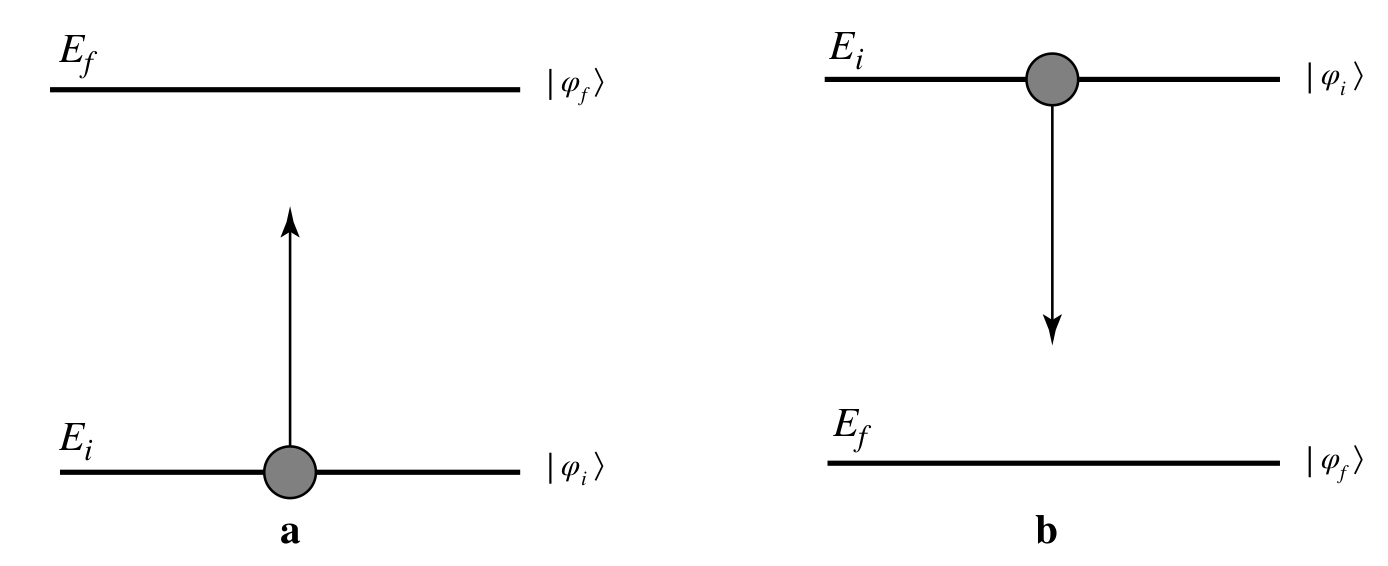
\includegraphics[width=0.64\textwidth]{images/state_transitions.png}
    \caption{Relative disposition of the energies $E_i$ and $E_f$ associated with the states $\ket{\phi_i}$ and $\ket{\phi_f}$. If $E_i < E_f$, (fig. a), the $\ket{\phi_i} \to \ket{\phi_f}$ transition occurs through absorption of an energy quantum $\hbar \omega$. If, on the other hand $E_i> E_f$ (fig. b), the transition occurs through induced emission of an energy quantum $\hbar \omega$.}
    \label{fig:state_transitions}
\end{figure}

From now, we will consider the case $\omega \to \omega_{fi}$ only, however the analysis for $\omega \to- \omega_{fi}$ can be made analogously.

Plotting $\mathcal{P}_{if}^{\omega\to\omega_{fi}}(t;\omega)$ as a function of $\omega$ for a specific time yields the curve shown in \textbf{Figure \ref{fig:P_if}}. We can see that when $\omega \simeq \omega_{fi}$, a resonance appears whose intensity is proportional to $t^2$ and whose width is inversely proportional to $t$. The probability of transition is greatest when the driving frequency $\omega$ is closest to the natural frequency $\omega_{if}$. It is also larger the longer the system is exposed to the perturbation.
\begin{figure}[htbp]
    \centering
    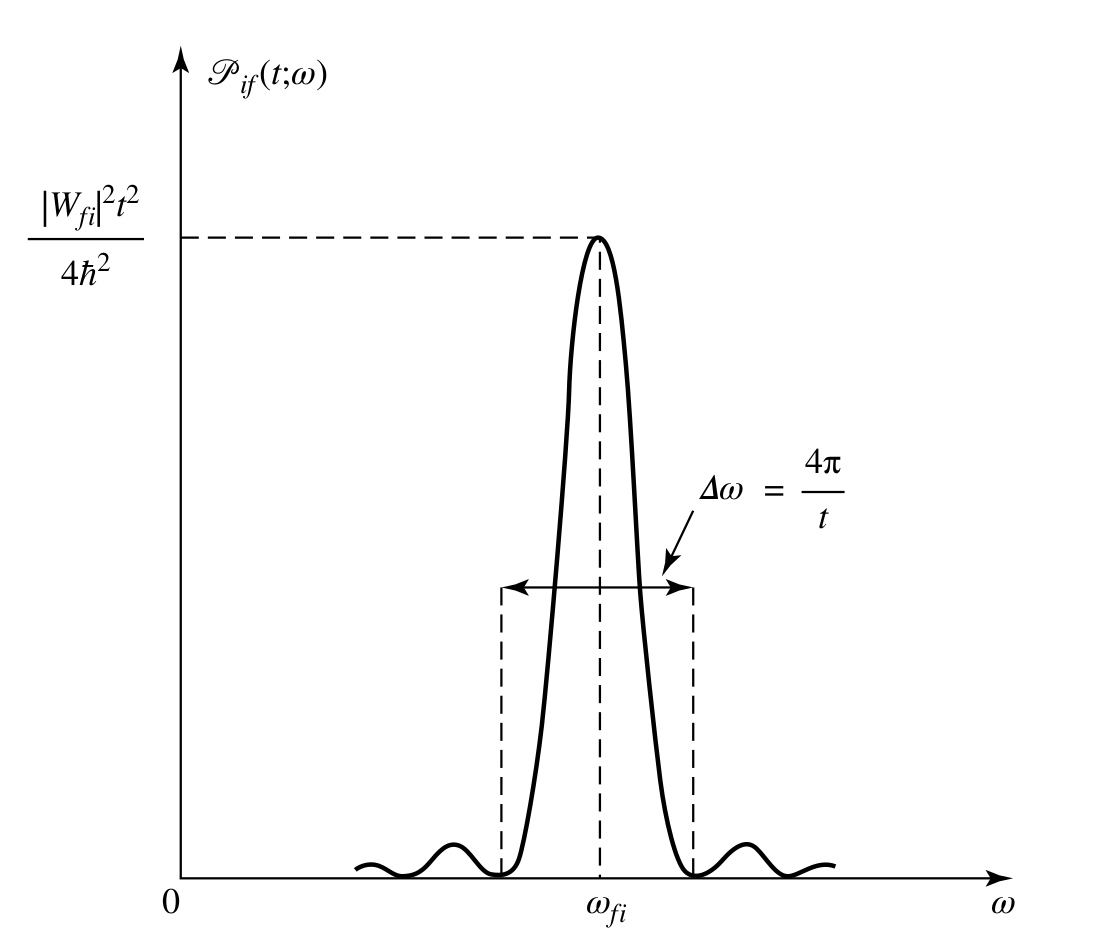
\includegraphics[width=0.8\textwidth]{images/P_if.png}
    \caption{Variation of the first order transition probability $\mathcal{P}_{if}(t;\omega)$ for $\omega \to \omega_{fi}$ as a function of $\omega$ for a fixed time $t$.}
    \label{fig:P_if}
\end{figure}

Note that, as the limit when $t\to\infty$, we have:
\begin{equation}
    \lim_{t\to\infty} \left(\frac{\sin(a t )}{ a}\right)^2 = \pi t \delta(a )
\end{equation}
Therefore, in our case:
\begin{equation}
    \lim_{t\to \infty} \mathcal{P}_{if}(t;\omega) = \frac{\left|{H_p}_{fi}\right|^2}{4\hbar^2}\lim_{t\to \infty}\left(\frac{\sin\frac{(\omega_{fi}-\omega)t}{2}}{\frac{\omega_{fi} - \omega}{2}} \right)^2 = \frac{\left|{H_p}_{fi}\right|^2}{4\hbar^2}\ \pi t\ \delta\left(\frac{\omega_{fi} - \omega}{2}\right)
\end{equation}

\subsubsection{Limits to the first order calculation}

If we look at the plot in \textbf{Figure \ref{fig:P_if}}, it is clear that there must be some limits to the application of the first order approximation. For instance, if we take a look at the expression of the maximum probability, we can see that it depends on time:
\begin{equation}
    \max \left(\mathcal{P}_{if}(t;\omega)\right) = \frac{\left|{H_p}_{fi}\right|^2t^2}{4\hbar^2},
\end{equation}
and that it goes to infinity at $t\to \infty$. This is clearly absurd, as probability can never go above $1$. In practice, for the first order approximation to be valid at resonance, it must be smaller than $1$. That is:
\begin{equation}\label{condition_1}
    t\ll\frac{\hbar }{\left|{H_p}_{fi}\right|}
\end{equation}

Furthermore, resonance will not take place unless the perturbation has had enough time to appear to the system as sinusoidal (in other words, it needs to perform a few oscillations for the system to perceive the perturbation as sinusoidal). This condition can  be expressed as:
\begin{equation}
    2|\omega_{fi}|\gg \Delta \omega,
\end{equation}
where $\Delta \omega = \frac{4\pi}{t}$ is the width of the resonant part in \textbf{Figure \ref{fig:P_if}}. The condition then becomes:
\begin{equation}\label{condition_2}
    \cancel{2}|\omega_{fi}|\gg \frac{\cancel{4\pi}}{t}\quad\longrightarrow\quad t \gg \frac{1}{\omega_{fi}}
\end{equation}
Therefore, combining the conditions from \textbf{Equation \ref{condition_1}} and \textbf{Equation \ref{condition_2}}, we obtain:
\begin{equation}
    \frac{1}{\omega_{fi}} \ll \frac{1}{\left|{H_p}_{fi}\right|}
\end{equation}

\subsubsection{Coupling between discrete states: Rabi's formula}

In this section, we will study the oscillations of a system between two discrete states when they are exposed to a sinusoidal resonant perturbation for a long time, for which the previous limiting conditions are not met. 

For these cases, as the first order solution is insufficient, in principle it would be possible to simply find higher order terms to obtain a better expression. However, such a method would lead to unnecessarily long calculations. In this section, we shall see that it is possible to solve the problem in a quicker and more elegant way by considering the fact that the resonance condition implies that only the two discrete states $\ket{\phi_i}$ and $\ket{\phi_f}$ are effetively coupled by the perturbation. In other words, the only possible transitions (with non-negligible probability) are between these two states. 

Back in \textbf{Section \ref{sec:time-dep-pert-thry}}, we replaced all the coefficients $b_k(t)$ of \textbf{Equation \ref{eq:time_dependent_perturbation_2}} by their expansion in $\lambda$:
\begin{equation}
    b_k(t) = \sum_{q=0}^\infty \lambda^q b_k^{(q)}(t),
\end{equation}
In this case, we will simply neglect all terms $k \neq i, f$ and leave $b_i(t)$ and $b_f(t)$ as they are:
\begin{equation}
    \begin{split}
        i \hbar\frac{db_i(t)}{dt} &= \lambda\sum_{k} e^{i\omega_{ik}t}W_{ik}(t)b_k(t) =\\
        &= \cancel{\lambda\sum_{k\neq i,f} e^{i\omega_{ik}t}W_{ik}(t)b_k(t)} + e^{i\omega_{ii}t} {H_p}_{ii}(t)b_i (t) + e^{i\omega_{if}t} {H_p}_{if}(t)b_f (t),
    \end{split}
\end{equation}
where we have used that $H_p(t) = \lambda W(t)$. Since the perturbation is sinusoidal, we have $H_p(t) = H_p \sin \omega t$. Therefore, using this and the fact that $\omega_{if} = -\omega_{fi}$:
\begin{equation}
    \begin{split}
        i \hbar\frac{db_i(t)}{dt} &= \cancelto{1}{e^{i\omega_{ii}t}} {H_p}_{ii}\sin(\omega t)b_i (t) + e^{-i\omega_{fi}t} {H_p}_{if}\sin(\omega t)b_f (t) =\\
        &= {H_p}_{ii}\left(\frac{e^{i\omega t}- e^{-i\omega t}}{2i}\right)b_i (t) + e^{-i\omega_{fi}t} {H_p}_{if}\left(\frac{e^{i\omega t}- e^{-i\omega t}}{2i}\right)b_f (t) =\\
        &= \frac{1}{2i}\left\{{H_p}_{ii}\left(e^{i\omega t}- e^{-i\omega t}\right)b_i (t) + e^{-i\omega_{fi}t} {H_p}_{if}\left(e^{i\omega t}- e^{-i\omega t}\right)b_f (t)\right\} =\\
        &= \frac{1}{2i}\left\{{H_p}_{ii} b_i (t) \left(e^{i\omega t}- e^{-i\omega t}\right) + {H_p}_{if}b_f (t) \left(e^{i(\omega - \omega_{fi}) t}- e^{-i(\omega + \omega_{fi}) t}\right)\right\}\\
    \end{split}
\end{equation}

Finally, if we do the same for $b_f(t)$, we obtain the following system of differential equations:
\begin{equation}
    \left\{\ 
    \begin{aligned}
        i \hbar\frac{db_i(t)}{dt} &= \frac{1}{2i}\left\{{H_p}_{ii} b_i (t) \left(e^{i\omega t}- e^{-i\omega t}\right) + {H_p}_{if}b_f (t) \left(e^{i(\omega - \omega_{fi}) t}- e^{-i(\omega + \omega_{fi}) t}\right)\right\}\\
        i \hbar\frac{db_f(t)}{dt} &= \frac{1}{2i}\left\{{H_p}_{fi}b_i (t) \left(e^{i(\omega + \omega_{if}) t}- e^{-i(\omega - \omega_{if}) t}\right) + {H_p}_{ff} b_f (t) \left(e^{i\omega t}- e^{-i\omega t}\right)\right\}
    \end{aligned}\right.
\end{equation}

On the right-hand side of these equations, certain coefficients of $b_i(t)$ and $b_f(t)$ are proportional to $e^{\pm i(\omega-\omega_{fi})t}$, so they oscillate slowly in time when $\omega\simeq \omega_{fi}$. On the other hand, the coefficients proportional to either $e^{\pm i\omega t}$ or $e^{\pm i(\omega+\omega_{fi})t}$ oscillate much more rapidly. Here, we will use the so called ``secular approximation'', which consists in neglecting the second type of terms, which average to zero when integrated over a large number of periods. The remaining ones (called ``secular terms'') are then those whose coefficients are reduced to constants for $\omega = \omega_{fi}$.

Note that, for the preceding argument to be valid, it is necessary for the temporal variation of a term $e^{i\omega t}b_{i,f}(t)$ to be due principally to the exponential, and not to the component $b_{i,f}(t)$. Since $\omega$ is very close to $\omega_{fi}$, this means that $b_{i,f}(t)$ must not vary significantly over a time interval of the order of $1/|\omega_{fi}|$. This is indeed true with the assumptions we have made, that is, with $H_p \ll H_0$. The variations of $b_{i,f}(t)$ (which are constants if $H_p= 0$) are due to the presence of the perturbation $H_p$, and are appreciable for times of the order of $\hbar / |{H_p}_{if}|$. Since, by hypothesis ${H_p}_{if}\ll\hbar |\omega_{fi}|$, this time is much greater $1/|\omega_{fi}|$.

In conclusion, the secular approximation leads to the following system of equations:
\begin{equation}
    \left\{\ 
    \begin{aligned}
        \frac{db_i(t)}{dt} &= -\frac{1}{2\hbar}\ e^{i(\omega - \omega_{fi}) t}{H_p}_{if}b_f (t)\\
        \frac{db_f(t)}{dt} &= \frac{1}{2\hbar}\ e^{-i(\omega - \omega_{if}) t}{H_p}_{fi}b_i (t) 
    \end{aligned}\right.,
\end{equation}
whose solution gives \textbf{Rabi's formula}, defined below:
\begin{definition}
    Rabi's formula gives the probability of a system in an initial state $\ket{\phi_i}$ to transition to a state $\ket{\phi_f}$ when submitted to a resonant perturbation $H_p(t) = H_p \sin(\omega t)$, where $\omega \simeq \omega_{fi}$. It is given by the expression:
    \begin{equation}
        \mathcal{P}_{if}(t;\omega) = \frac{|{H_p}_{if}|^2}{|{H_p}_{if}|^2 + \hbar^2(\omega-\omega_{fi})^2} \sin \left[\frac{t}{2}\sqrt{\frac{|{H_p}_{fi}|^2}{\hbar} + (\omega-\omega_{fi})^2}\ \right]
    \end{equation}
\end{definition}

Rabi's formula measures the magnitude of the resonance phenomenon. Note that, when $\omega=\omega_{fi}$, however small the perturbation is, it can cause the system to move completely to the final state $\ket{\phi_f}$, irrespective of the magnitude of $H_p$. The only effect of the magnitude of $H_p$ is to make the transition faster (for larger $H_p$) or slower (for smaller $H_p$).

Note also that the probability is an oscillating function of time. For certain periodic time intervals, the probability of transition is zero, and the system has returned to the initial state $\ket{\phi_i}$

Finally, we can see that this expression is valid both for $t\to \infty$ and $t\to 0$, and it remains always bounded between $0$ and $1$.